\documentclass[tikz]{standalone}
\usepackage{pgfplots}
\usepackage{amsmath}
\pgfplotsset{compat=1.18}

\begin{document}

% Site 1 (DLE) - Deposit Belief Uncertainty Evolution
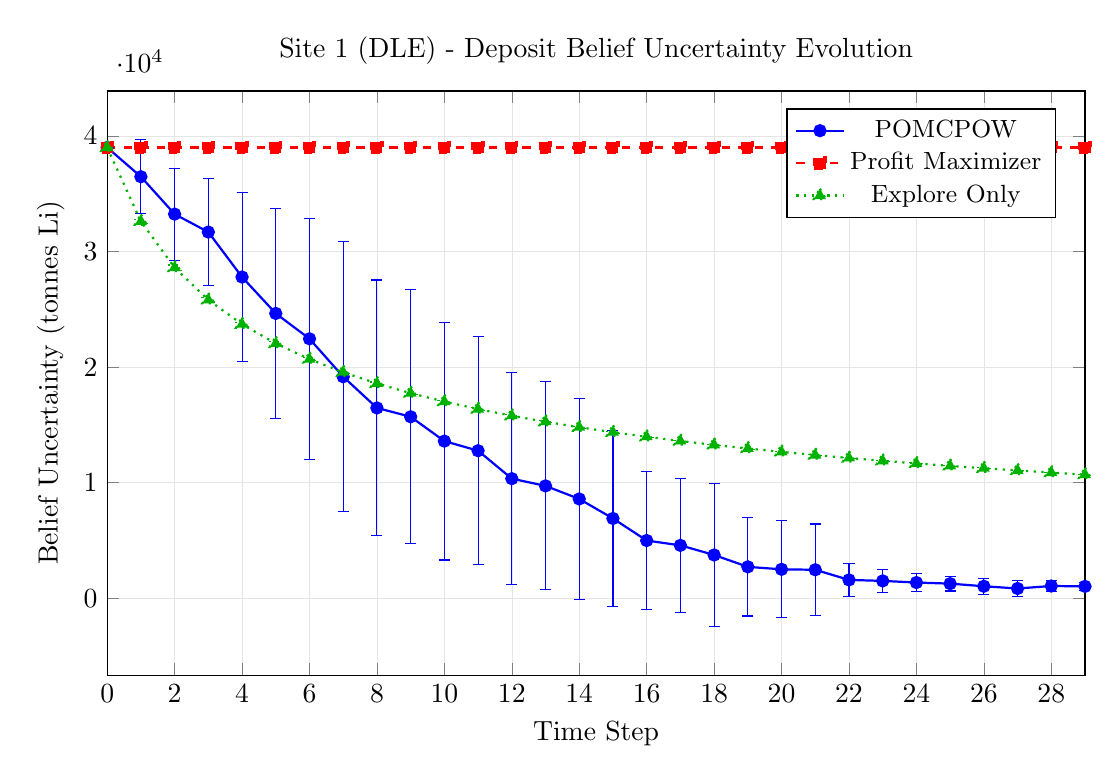
\begin{tikzpicture}
\begin{axis}[
    width=14cm,
    height=9cm,
    title={Site 1 (DLE) - Deposit Belief Uncertainty Evolution},
    xlabel={Time Step},
    ylabel={Belief Uncertainty (tonnes Li)},
    xmin=0, xmax=29,
    grid=major,
    grid style={line width=.2pt, draw=gray!20},
    legend pos=north east,
    legend style={font=\small}
]

% POMCPOW - Site 1 with error bars
\addplot[blue, thick, solid, mark=*, mark size=2pt, error bars/.cd, y dir=both, y explicit] coordinates {
    (0, 39000.0) +- (0, 0.0) (1, 36469.53) +- (0, 3208.09) (2, 33235.57) +- (0, 3979.75) (3, 31680.49) +- (0, 4657.39) (4, 27792.12) +- (0, 7304.34) (5, 24642.41) +- (0, 9061.22) (6, 22448.81) +- (0, 10425.32) (7, 19168.23) +- (0, 11664.22) (8, 16470.92) +- (0, 11068.11) (9, 15704.61) +- (0, 10996.26) (10, 13599.82) +- (0, 10280.82) (11, 12769.66) +- (0, 9859.71) (12, 10353.35) +- (0, 9192.41) (13, 9726.82) +- (0, 8999.78) (14, 8597.62) +- (0, 8671.37) (15, 6908.5) +- (0, 7598.05) (16, 5000.02) +- (0, 5947.64) (17, 4583.38) +- (0, 5776.84) (18, 3750.79) +- (0, 6178.17) (19, 2725.31) +- (0, 4249.71) (20, 2509.53) +- (0, 4197.56) (21, 2470.6) +- (0, 3959.92) (22, 1595.11) +- (0, 1441.19) (23, 1509.56) +- (0, 997.55) (24, 1367.21) +- (0, 767.07) (25, 1272.76) +- (0, 637.88) (26, 1044.8) +- (0, 686.14) (27, 850.95) +- (0, 709.76) (28, 1068.21) +- (0, 464.73) (29, 1034.04) +- (0, 317.48)
};
\addlegendentry{POMCPOW}

% ProfitMaximizer - Site 1 with error bars
\addplot[red, thick, dashed, mark=square*, mark size=2pt, error bars/.cd, y dir=both, y explicit] coordinates {
    (0, 39000.0) +- (0, 0.0) (1, 39000.0) +- (0, 0.0) (2, 39000.0) +- (0, 0.0) (3, 39000.0) +- (0, 0.0) (4, 39000.0) +- (0, 0.0) (5, 39000.0) +- (0, 0.0) (6, 39000.0) +- (0, 0.0) (7, 39000.0) +- (0, 0.0) (8, 39000.0) +- (0, 0.0) (9, 39000.0) +- (0, 0.0) (10, 39000.0) +- (0, 0.0) (11, 39000.0) +- (0, 0.0) (12, 39000.0) +- (0, 0.0) (13, 39000.0) +- (0, 0.0) (14, 39000.0) +- (0, 0.0) (15, 39000.0) +- (0, 0.0) (16, 39000.0) +- (0, 0.0) (17, 39000.0) +- (0, 0.0) (18, 39000.0) +- (0, 0.0) (19, 39000.0) +- (0, 0.0) (20, 39000.0) +- (0, 0.0) (21, 39000.0) +- (0, 0.0) (22, 39000.0) +- (0, 0.0) (23, 39000.0) +- (0, 0.0) (24, 39000.0) +- (0, 0.0) (25, 39000.0) +- (0, 0.0) (26, 39000.0) +- (0, 0.0) (27, 39000.0) +- (0, 0.0) (28, 39000.0) +- (0, 0.0) (29, 39000.0) +- (0, 0.0)
};
\addlegendentry{Profit Maximizer}

% ExploreOnly - Site 1 with error bars
\addplot[green!70!black, thick, dotted, mark=triangle*, mark size=2.5pt, error bars/.cd, y dir=both, y explicit] coordinates {
    (0, 39000.0) +- (0, 0.0) (1, 32603.62) +- (0, 147.45) (2, 28603.5) +- (0, 234.62) (3, 25815.96) +- (0, 185.08) (4, 23709.78) +- (0, 158.29) (5, 22043.61) +- (0, 153.03) (6, 20689.06) +- (0, 135.1) (7, 19555.29) +- (0, 127.81) (8, 18587.47) +- (0, 129.69) (9, 17748.05) +- (0, 139.54) (10, 17018.58) +- (0, 124.97) (11, 16372.27) +- (0, 112.88) (12, 15794.47) +- (0, 102.53) (13, 15273.93) +- (0, 93.43) (14, 14801.74) +- (0, 85.4) (15, 14370.77) +- (0, 78.64) (16, 13975.46) +- (0, 72.48) (17, 13611.07) +- (0, 67.07) (18, 13273.78) +- (0, 62.32) (19, 12960.38) +- (0, 58.13) (20, 12668.19) +- (0, 54.34) (21, 12394.91) +- (0, 50.95) (22, 12138.59) +- (0, 47.89) (23, 11897.55) +- (0, 45.13) (24, 11670.31) +- (0, 42.62) (25, 11455.62) +- (0, 40.34) (26, 11252.36) +- (0, 38.25) (27, 11059.55) +- (0, 36.34) (28, 10876.32) +- (0, 34.58) (29, 10701.9) +- (0, 32.96)
};
\addlegendentry{Explore Only}

\end{axis}
\end{tikzpicture}

\vspace{1cm}

% Site 2 (DLE) - Deposit Belief Uncertainty Evolution
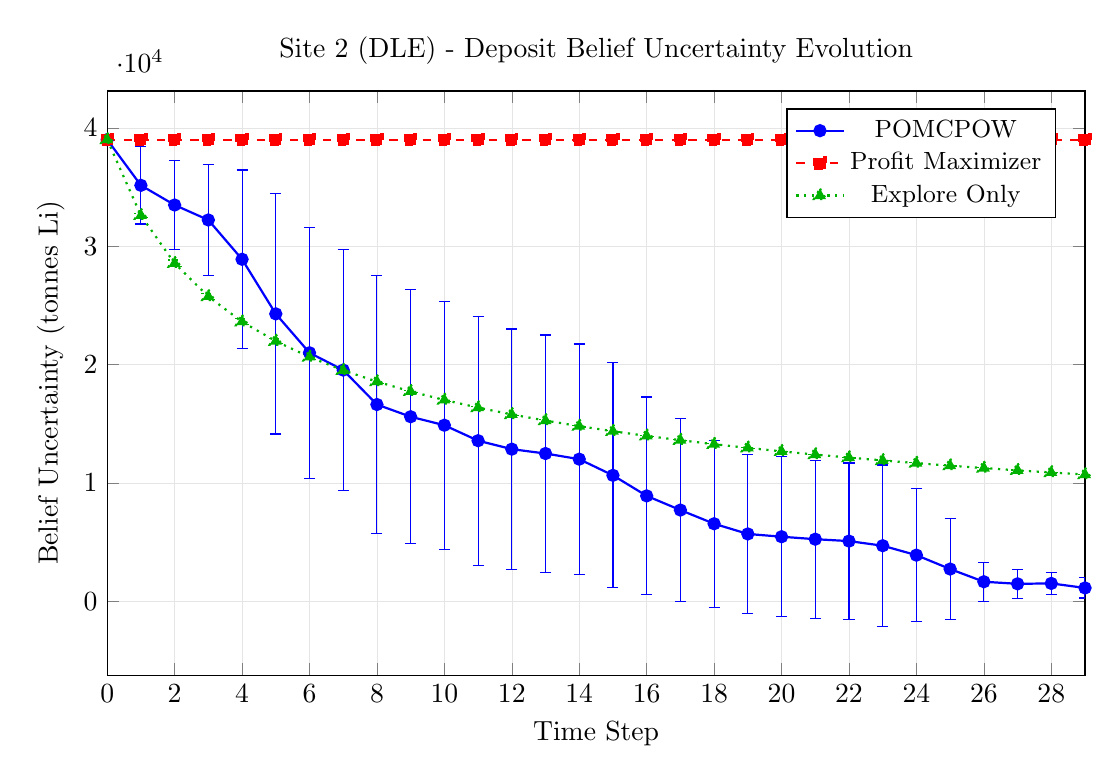
\begin{tikzpicture}
\begin{axis}[
    width=14cm,
    height=9cm,
    title={Site 2 (DLE) - Deposit Belief Uncertainty Evolution},
    xlabel={Time Step},
    ylabel={Belief Uncertainty (tonnes Li)},
    xmin=0, xmax=29,
    grid=major,
    grid style={line width=.2pt, draw=gray!20},
    legend pos=north east,
    legend style={font=\small}
]

% POMCPOW - Site 2 with error bars
\addplot[blue, thick, solid, mark=*, mark size=2pt, error bars/.cd, y dir=both, y explicit] coordinates {
    (0, 39000.0) +- (0, 0.0) (1, 35137.33) +- (0, 3267.3) (2, 33475.21) +- (0, 3788.91) (3, 32209.86) +- (0, 4671.85) (4, 28890.11) +- (0, 7539.79) (5, 24276.54) +- (0, 10153.55) (6, 20988.52) +- (0, 10595.24) (7, 19528.0) +- (0, 10158.98) (8, 16616.22) +- (0, 10919.09) (9, 15584.51) +- (0, 10716.53) (10, 14867.41) +- (0, 10469.29) (11, 13560.32) +- (0, 10527.74) (12, 12844.95) +- (0, 10157.53) (13, 12474.6) +- (0, 10019.14) (14, 11998.71) +- (0, 9734.7) (15, 10631.14) +- (0, 9507.8) (16, 8896.54) +- (0, 8359.0) (17, 7697.91) +- (0, 7716.65) (18, 6541.95) +- (0, 7041.83) (19, 5679.62) +- (0, 6698.02) (20, 5444.74) +- (0, 6763.63) (21, 5236.97) +- (0, 6675.44) (22, 5076.35) +- (0, 6601.81) (23, 4685.98) +- (0, 6818.2) (24, 3887.55) +- (0, 5619.12) (25, 2714.14) +- (0, 4243.78) (26, 1641.55) +- (0, 1645.61) (27, 1465.88) +- (0, 1236.93) (28, 1499.12) +- (0, 906.61) (29, 1116.95) +- (0, 845.68)
};
\addlegendentry{POMCPOW}

% ProfitMaximizer - Site 2 with error bars
\addplot[red, thick, dashed, mark=square*, mark size=2pt, error bars/.cd, y dir=both, y explicit] coordinates {
    (0, 39000.0) +- (0, 0.0) (1, 39000.0) +- (0, 0.0) (2, 39000.0) +- (0, 0.0) (3, 39000.0) +- (0, 0.0) (4, 39000.0) +- (0, 0.0) (5, 39000.0) +- (0, 0.0) (6, 39000.0) +- (0, 0.0) (7, 39000.0) +- (0, 0.0) (8, 39000.0) +- (0, 0.0) (9, 39000.0) +- (0, 0.0) (10, 39000.0) +- (0, 0.0) (11, 39000.0) +- (0, 0.0) (12, 39000.0) +- (0, 0.0) (13, 39000.0) +- (0, 0.0) (14, 39000.0) +- (0, 0.0) (15, 39000.0) +- (0, 0.0) (16, 39000.0) +- (0, 0.0) (17, 39000.0) +- (0, 0.0) (18, 39000.0) +- (0, 0.0) (19, 39000.0) +- (0, 0.0) (20, 39000.0) +- (0, 0.0) (21, 39000.0) +- (0, 0.0) (22, 39000.0) +- (0, 0.0) (23, 39000.0) +- (0, 0.0) (24, 39000.0) +- (0, 0.0) (25, 39000.0) +- (0, 0.0) (26, 39000.0) +- (0, 0.0) (27, 39000.0) +- (0, 0.0) (28, 39000.0) +- (0, 0.0) (29, 39000.0) +- (0, 0.0)
};
\addlegendentry{Profit Maximizer}

% ExploreOnly - Site 2 with error bars
\addplot[green!70!black, thick, dotted, mark=triangle*, mark size=2.5pt, error bars/.cd, y dir=both, y explicit] coordinates {
    (0, 39000.0) +- (0, 0.0) (1, 32594.96) +- (0, 152.41) (2, 28548.17) +- (0, 278.37) (3, 25741.68) +- (0, 240.49) (4, 23610.49) +- (0, 266.91) (5, 21968.24) +- (0, 217.84) (6, 20628.67) +- (0, 180.84) (7, 19507.65) +- (0, 153.26) (8, 18551.58) +- (0, 132.05) (9, 17723.58) +- (0, 115.33) (10, 16997.41) +- (0, 101.86) (11, 16353.79) +- (0, 90.81) (12, 15778.16) +- (0, 81.62) (13, 15259.33) +- (0, 73.88) (14, 14788.54) +- (0, 67.29) (15, 14358.79) +- (0, 61.63) (16, 13964.46) +- (0, 56.72) (17, 13600.93) +- (0, 52.43) (18, 13264.4) +- (0, 48.65) (19, 12951.66) +- (0, 45.31) (20, 12660.06) +- (0, 42.33) (21, 12387.3) +- (0, 39.66) (22, 12131.45) +- (0, 37.27) (23, 11890.82) +- (0, 35.1) (24, 11663.97) +- (0, 33.14) (25, 11449.62) +- (0, 31.35) (26, 11246.68) +- (0, 29.72) (27, 11054.15) +- (0, 28.22) (28, 10871.19) +- (0, 26.85) (29, 10697.02) +- (0, 25.59)
};
\addlegendentry{Explore Only}

\end{axis}
\end{tikzpicture}

\vspace{1cm}

% Site 3 (Hard Rock Mining) - Deposit Belief Uncertainty Evolution
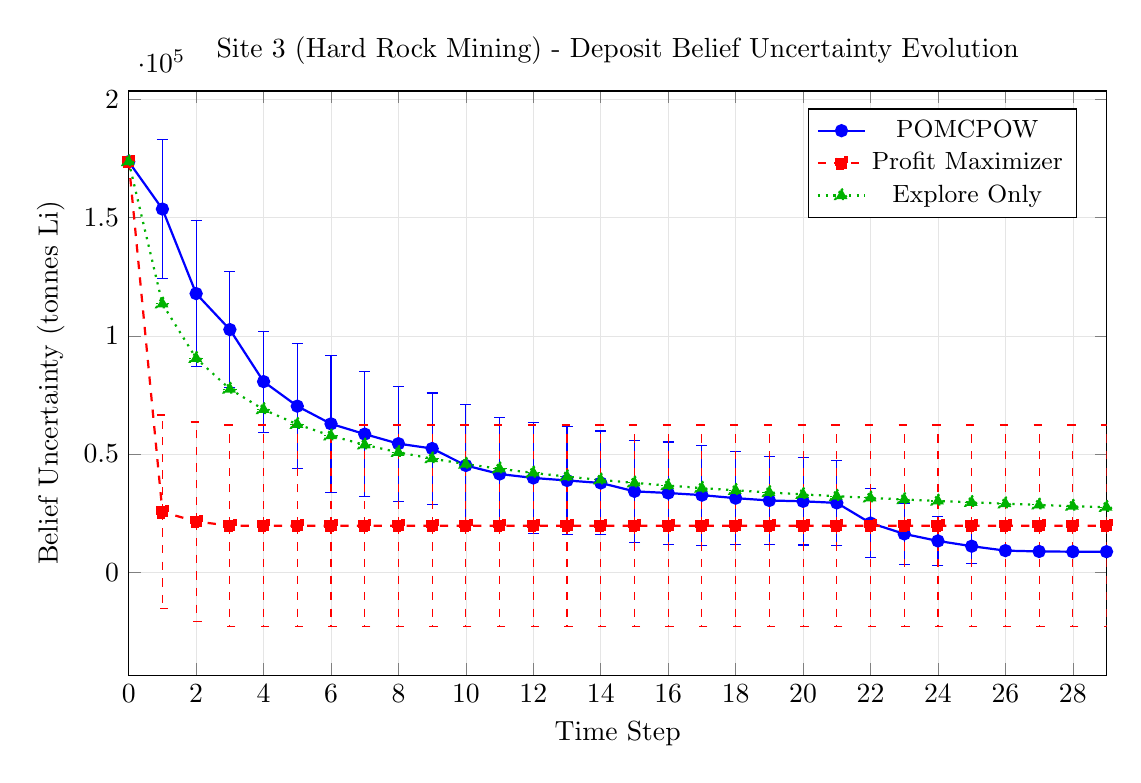
\begin{tikzpicture}
\begin{axis}[
    width=14cm,
    height=9cm,
    title={Site 3 (Hard Rock Mining) - Deposit Belief Uncertainty Evolution},
    xlabel={Time Step},
    ylabel={Belief Uncertainty (tonnes Li)},
    xmin=0, xmax=29,
    grid=major,
    grid style={line width=.2pt, draw=gray!20},
    legend pos=north east,
    legend style={font=\small}
]

% POMCPOW - Site 3 with error bars
\addplot[blue, thick, solid, mark=*, mark size=2pt, error bars/.cd, y dir=both, y explicit] coordinates {
    (0, 173756.0) +- (0, 0.0) (1, 153685.16) +- (0, 29380.7) (2, 117914.25) +- (0, 30749.94) (3, 102678.97) +- (0, 24492.31) (4, 80663.05) +- (0, 21379.49) (5, 70279.03) +- (0, 26336.99) (6, 62788.35) +- (0, 29051.92) (7, 58444.35) +- (0, 26556.44) (8, 54404.31) +- (0, 24379.29) (9, 52348.51) +- (0, 23518.95) (10, 45167.64) +- (0, 25823.71) (11, 41563.52) +- (0, 24005.49) (12, 39893.48) +- (0, 23408.35) (13, 38825.58) +- (0, 22721.09) (14, 37768.75) +- (0, 21989.18) (15, 34227.53) +- (0, 21588.22) (16, 33522.57) +- (0, 21603.57) (17, 32621.49) +- (0, 21153.65) (18, 31343.4) +- (0, 19769.92) (19, 30362.98) +- (0, 18731.25) (20, 30009.61) +- (0, 18468.2) (21, 29342.55) +- (0, 17972.52) (22, 20804.78) +- (0, 14737.9) (23, 16215.22) +- (0, 12779.48) (24, 13239.46) +- (0, 10403.44) (25, 11017.21) +- (0, 7232.3) (26, 9138.93) +- (0, 1373.34) (27, 8787.86) +- (0, 387.52) (28, 8687.8) +- (0, 0.0) (29, 8687.8) +- (0, 0.0)
};
\addlegendentry{POMCPOW}

% ProfitMaximizer - Site 3 with error bars
\addplot[red, thick, dashed, mark=square*, mark size=2pt, error bars/.cd, y dir=both, y explicit] coordinates {
    (0, 173756.0) +- (0, 0.0) (1, 25531.86) +- (0, 41004.97) (2, 21464.84) +- (0, 42130.08) (3, 19692.35) +- (0, 42620.43) (4, 19692.35) +- (0, 42620.43) (5, 19692.35) +- (0, 42620.43) (6, 19692.35) +- (0, 42620.43) (7, 19692.35) +- (0, 42620.43) (8, 19692.35) +- (0, 42620.43) (9, 19692.35) +- (0, 42620.43) (10, 19692.35) +- (0, 42620.43) (11, 19692.35) +- (0, 42620.43) (12, 19692.35) +- (0, 42620.43) (13, 19692.35) +- (0, 42620.43) (14, 19692.35) +- (0, 42620.43) (15, 19692.35) +- (0, 42620.43) (16, 19692.35) +- (0, 42620.43) (17, 19692.35) +- (0, 42620.43) (18, 19692.35) +- (0, 42620.43) (19, 19692.35) +- (0, 42620.43) (20, 19692.35) +- (0, 42620.43) (21, 19692.35) +- (0, 42620.43) (22, 19692.35) +- (0, 42620.43) (23, 19692.35) +- (0, 42620.43) (24, 19692.35) +- (0, 42620.43) (25, 19692.35) +- (0, 42620.43) (26, 19692.35) +- (0, 42620.43) (27, 19692.35) +- (0, 42620.43) (28, 19692.35) +- (0, 42620.43) (29, 19692.35) +- (0, 42620.43)
};
\addlegendentry{Profit Maximizer}

% ExploreOnly - Site 3 with error bars
\addplot[green!70!black, thick, dotted, mark=triangle*, mark size=2.5pt, error bars/.cd, y dir=both, y explicit] coordinates {
    (0, 173756.0) +- (0, 0.0) (1, 113543.45) +- (0, 0.1) (2, 90531.58) +- (0, 0.05) (3, 77508.74) +- (0, 0.03) (4, 68859.14) +- (0, 0.02) (5, 62580.16) +- (0, 0.02) (6, 57755.34) +- (0, 0.01) (7, 53898.1) +- (0, 0.01) (8, 50723.02) +- (0, 0.01) (9, 48050.15) +- (0, 0.01) (10, 45759.68) +- (0, 0.01) (11, 43768.34) +- (0, 0.01) (12, 42016.23) +- (0, 0.01) (13, 40458.98) +- (0, 0.0) (14, 39062.96) +- (0, 0.0) (15, 37802.14) +- (0, 0.0) (16, 36656.03) +- (0, 0.0) (17, 35608.21) +- (0, 0.0) (18, 34645.4) +- (0, 0.0) (19, 33756.69) +- (0, 0.0) (20, 32933.05) +- (0, 0.0) (21, 32166.89) +- (0, 0.0) (22, 31451.83) +- (0, 0.0) (23, 30782.43) +- (0, 0.0) (24, 30154.03) +- (0, 0.0) (25, 29562.6) +- (0, 0.0) (26, 29004.67) +- (0, 0.0) (27, 28477.18) +- (0, 0.0) (28, 27977.45) +- (0, 0.0) (29, 27503.15) +- (0, 0.0)
};
\addlegendentry{Explore Only}

\end{axis}
\end{tikzpicture}

\vspace{1cm}

% Site 4 (Hard Rock Mining) - Deposit Belief Uncertainty Evolution
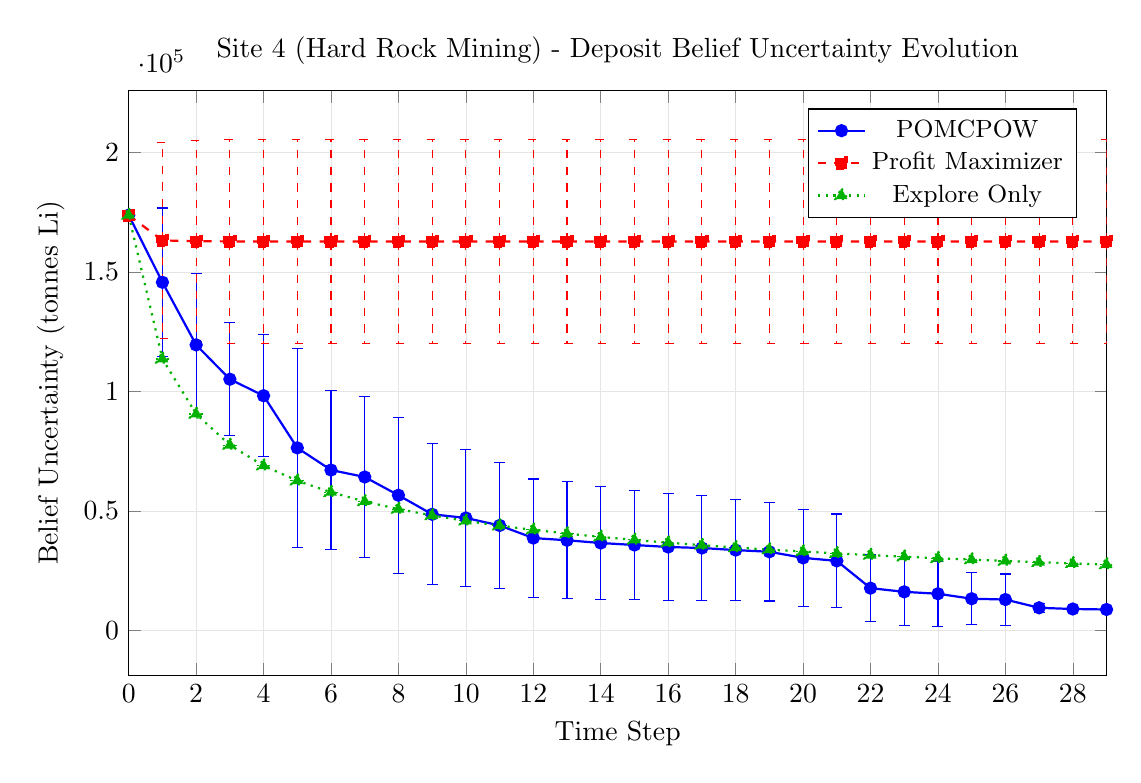
\begin{tikzpicture}
\begin{axis}[
    width=14cm,
    height=9cm,
    title={Site 4 (Hard Rock Mining) - Deposit Belief Uncertainty Evolution},
    xlabel={Time Step},
    ylabel={Belief Uncertainty (tonnes Li)},
    xmin=0, xmax=29,
    grid=major,
    grid style={line width=.2pt, draw=gray!20},
    legend pos=north east,
    legend style={font=\small}
]

% POMCPOW - Site 4 with error bars
\addplot[blue, thick, solid, mark=*, mark size=2pt, error bars/.cd, y dir=both, y explicit] coordinates {
    (0, 173756.0) +- (0, 0.0) (1, 145656.82) +- (0, 31093.62) (2, 119449.48) +- (0, 29846.77) (3, 105081.28) +- (0, 23598.05) (4, 98165.88) +- (0, 25562.21) (5, 76346.46) +- (0, 41646.99) (6, 67065.21) +- (0, 33381.35) (7, 64154.99) +- (0, 33522.98) (8, 56510.06) +- (0, 32634.95) (9, 48531.79) +- (0, 29483.65) (10, 47011.13) +- (0, 28776.9) (11, 43859.0) +- (0, 26248.08) (12, 38587.03) +- (0, 24731.69) (13, 37665.5) +- (0, 24423.52) (14, 36517.22) +- (0, 23712.17) (15, 35681.27) +- (0, 22889.66) (16, 34848.08) +- (0, 22211.12) (17, 34424.73) +- (0, 21847.2) (18, 33545.73) +- (0, 21172.61) (19, 32850.47) +- (0, 20602.4) (20, 30295.13) +- (0, 20386.63) (21, 29040.47) +- (0, 19625.66) (22, 17621.68) +- (0, 13935.4) (23, 16077.88) +- (0, 13944.49) (24, 15273.41) +- (0, 13663.1) (25, 13197.69) +- (0, 10880.01) (26, 12854.86) +- (0, 10687.82) (27, 9396.56) +- (0, 1870.55) (28, 8894.24) +- (0, 544.86) (29, 8687.8) +- (0, 0.0)
};
\addlegendentry{POMCPOW}

% ProfitMaximizer - Site 4 with error bars
\addplot[red, thick, dashed, mark=square*, mark size=2pt, error bars/.cd, y dir=both, y explicit] coordinates {
    (0, 173756.0) +- (0, 0.0) (1, 163168.56) +- (0, 41004.97) (2, 162878.06) +- (0, 42130.08) (3, 162751.45) +- (0, 42620.43) (4, 162751.45) +- (0, 42620.43) (5, 162751.45) +- (0, 42620.43) (6, 162751.45) +- (0, 42620.43) (7, 162751.45) +- (0, 42620.43) (8, 162751.45) +- (0, 42620.43) (9, 162751.45) +- (0, 42620.43) (10, 162751.45) +- (0, 42620.43) (11, 162751.45) +- (0, 42620.43) (12, 162751.45) +- (0, 42620.43) (13, 162751.45) +- (0, 42620.43) (14, 162751.45) +- (0, 42620.43) (15, 162751.45) +- (0, 42620.43) (16, 162751.45) +- (0, 42620.43) (17, 162751.45) +- (0, 42620.43) (18, 162751.45) +- (0, 42620.43) (19, 162751.45) +- (0, 42620.43) (20, 162751.45) +- (0, 42620.43) (21, 162751.45) +- (0, 42620.43) (22, 162751.45) +- (0, 42620.43) (23, 162751.45) +- (0, 42620.43) (24, 162751.45) +- (0, 42620.43) (25, 162751.45) +- (0, 42620.43) (26, 162751.45) +- (0, 42620.43) (27, 162751.45) +- (0, 42620.43) (28, 162751.45) +- (0, 42620.43) (29, 162751.45) +- (0, 42620.43)
};
\addlegendentry{Profit Maximizer}

% ExploreOnly - Site 4 with error bars
\addplot[green!70!black, thick, dotted, mark=triangle*, mark size=2.5pt, error bars/.cd, y dir=both, y explicit] coordinates {
    (0, 173756.0) +- (0, 0.0) (1, 113543.45) +- (0, 0.15) (2, 90531.58) +- (0, 0.07) (3, 77508.74) +- (0, 0.05) (4, 68859.14) +- (0, 0.03) (5, 62580.16) +- (0, 0.02) (6, 57755.34) +- (0, 0.02) (7, 53898.1) +- (0, 0.02) (8, 50723.02) +- (0, 0.01) (9, 48050.15) +- (0, 0.01) (10, 45759.68) +- (0, 0.01) (11, 43768.34) +- (0, 0.01) (12, 42016.23) +- (0, 0.01) (13, 40458.98) +- (0, 0.01) (14, 39062.96) +- (0, 0.01) (15, 37802.14) +- (0, 0.01) (16, 36656.03) +- (0, 0.0) (17, 35608.21) +- (0, 0.0) (18, 34645.4) +- (0, 0.0) (19, 33756.69) +- (0, 0.0) (20, 32933.05) +- (0, 0.0) (21, 32166.89) +- (0, 0.0) (22, 31451.83) +- (0, 0.0) (23, 30782.43) +- (0, 0.0) (24, 30154.03) +- (0, 0.0) (25, 29562.6) +- (0, 0.0) (26, 29004.67) +- (0, 0.0) (27, 28477.18) +- (0, 0.0) (28, 27977.45) +- (0, 0.0) (29, 27503.15) +- (0, 0.0)
};
\addlegendentry{Explore Only}

\end{axis}
\end{tikzpicture}

\vspace{1cm}

% Price Belief Uncertainty Evolution
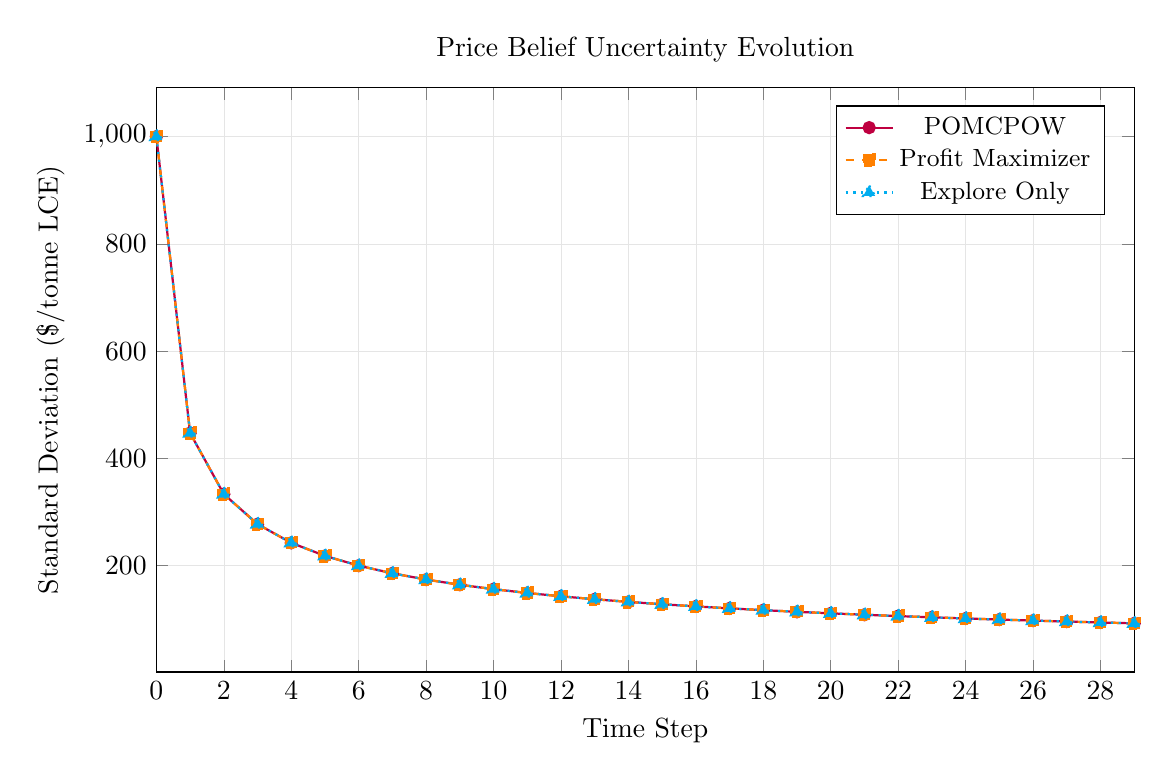
\begin{tikzpicture}
\begin{axis}[
    width=14cm,
    height=9cm,
    title={Price Belief Uncertainty Evolution},
    xlabel={Time Step},
    ylabel={Standard Deviation (\$/tonne LCE)},
    xmin=0, xmax=29,
    grid=major,
    grid style={line width=.2pt, draw=gray!20},
    legend pos=north east,
    legend style={font=\small}
]

% POMCPOW Price Uncertainty
\addplot[purple, thick, solid, mark=*, mark size=2pt] coordinates {
    (0, 1000.0) (1, 447.21) (2, 333.33) (3, 277.35) (4, 242.54) (5, 218.22) (6, 200.0) (7, 185.7) (8, 174.08) (9, 164.4) (10, 156.17) (11, 149.07) (12, 142.86) (13, 137.36) (14, 132.45) (15, 128.04) (16, 124.03) (17, 120.39) (18, 117.04) (19, 113.96) (20, 111.11) (21, 108.47) (22, 106.0) (23, 103.7) (24, 101.53) (25, 99.5) (26, 97.59) (27, 95.78) (28, 94.07) (29, 92.45)
};
\addlegendentry{POMCPOW}

% ProfitMaximizer Price Uncertainty
\addplot[orange, thick, dashed, mark=square*, mark size=2pt] coordinates {
    (0, 1000.0) (1, 447.21) (2, 333.33) (3, 277.35) (4, 242.54) (5, 218.22) (6, 200.0) (7, 185.7) (8, 174.08) (9, 164.4) (10, 156.17) (11, 149.07) (12, 142.86) (13, 137.36) (14, 132.45) (15, 128.04) (16, 124.03) (17, 120.39) (18, 117.04) (19, 113.96) (20, 111.11) (21, 108.47) (22, 106.0) (23, 103.7) (24, 101.53) (25, 99.5) (26, 97.59) (27, 95.78) (28, 94.07) (29, 92.45)
};
\addlegendentry{Profit Maximizer}

% ExploreOnly Price Uncertainty
\addplot[cyan, thick, dotted, mark=triangle*, mark size=2.5pt] coordinates {
    (0, 1000.0) (1, 447.21) (2, 333.33) (3, 277.35) (4, 242.54) (5, 218.22) (6, 200.0) (7, 185.7) (8, 174.08) (9, 164.4) (10, 156.17) (11, 149.07) (12, 142.86) (13, 137.36) (14, 132.45) (15, 128.04) (16, 124.03) (17, 120.39) (18, 117.04) (19, 113.96) (20, 111.11) (21, 108.47) (22, 106.0) (23, 103.7) (24, 101.53) (25, 99.5) (26, 97.59) (27, 95.78) (28, 94.07) (29, 92.45)
};
\addlegendentry{Explore Only}

\end{axis}
\end{tikzpicture}

\vspace{1cm}

% Demand Belief Uncertainty Evolution
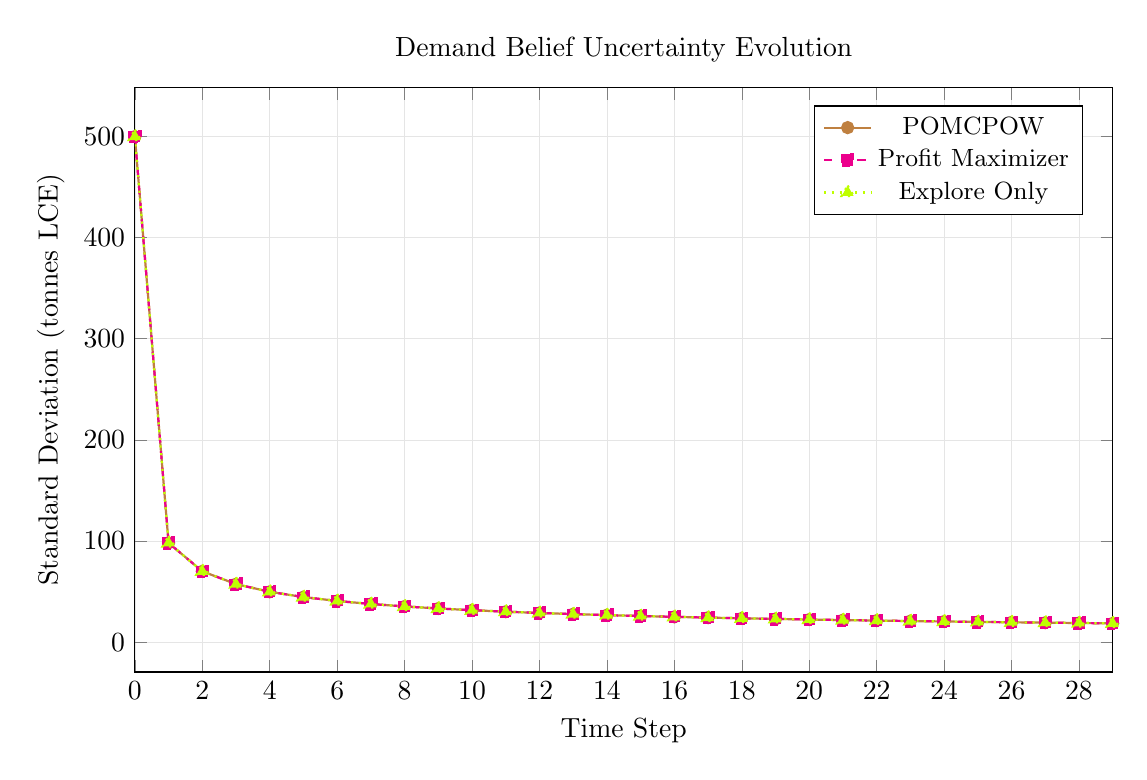
\begin{tikzpicture}
\begin{axis}[
    width=14cm,
    height=9cm,
    title={Demand Belief Uncertainty Evolution},
    xlabel={Time Step},
    ylabel={Standard Deviation (tonnes LCE)},
    xmin=0, xmax=29,
    grid=major,
    grid style={line width=.2pt, draw=gray!20},
    legend pos=north east,
    legend style={font=\small}
]

% POMCPOW Demand Uncertainty
\addplot[brown, thick, solid, mark=*, mark size=2pt] coordinates {
    (0, 500.0) (1, 98.06) (2, 70.01) (3, 57.35) (4, 49.75) (5, 44.54) (6, 40.69) (7, 37.69) (8, 35.27) (9, 33.26) (10, 31.56) (11, 30.1) (12, 28.82) (13, 27.69) (14, 26.69) (15, 25.79) (16, 24.97) (17, 24.23) (18, 23.54) (19, 22.92) (20, 22.34) (21, 21.8) (22, 21.3) (23, 20.83) (24, 20.4) (25, 19.98) (26, 19.6) (27, 19.23) (28, 18.88) (29, 18.56)
};
\addlegendentry{POMCPOW}

% ProfitMaximizer Demand Uncertainty
\addplot[magenta, thick, dashed, mark=square*, mark size=2pt] coordinates {
    (0, 500.0) (1, 98.06) (2, 70.01) (3, 57.35) (4, 49.75) (5, 44.54) (6, 40.69) (7, 37.69) (8, 35.27) (9, 33.26) (10, 31.56) (11, 30.1) (12, 28.82) (13, 27.69) (14, 26.69) (15, 25.79) (16, 24.97) (17, 24.23) (18, 23.54) (19, 22.92) (20, 22.34) (21, 21.8) (22, 21.3) (23, 20.83) (24, 20.4) (25, 19.98) (26, 19.6) (27, 19.23) (28, 18.88) (29, 18.56)
};
\addlegendentry{Profit Maximizer}

% ExploreOnly Demand Uncertainty
\addplot[lime, thick, dotted, mark=triangle*, mark size=2.5pt] coordinates {
    (0, 500.0) (1, 98.06) (2, 70.01) (3, 57.35) (4, 49.75) (5, 44.54) (6, 40.69) (7, 37.69) (8, 35.27) (9, 33.26) (10, 31.56) (11, 30.1) (12, 28.82) (13, 27.69) (14, 26.69) (15, 25.79) (16, 24.97) (17, 24.23) (18, 23.54) (19, 22.92) (20, 22.34) (21, 21.8) (22, 21.3) (23, 20.83) (24, 20.4) (25, 19.98) (26, 19.6) (27, 19.23) (28, 18.88) (29, 18.56)
};
\addlegendentry{Explore Only}

\end{axis}
\end{tikzpicture}

\end{document}
